Rancangan integrasi dengan sistem FHIR dapat dilihat pada Gambar 4.6. Sistem ini akan terintegrasi dengan sistem FHIR untuk mendapatkan data login dari pasien. Data login ini kemudian akan digunakan sebagai input untuk melakukan analisis risiko autentikasi.
\begin{figure}[H]
    \centering
    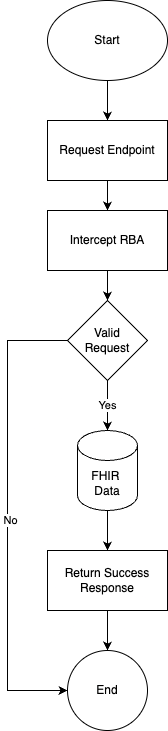
\includegraphics[width=0.2\textwidth]{BAB_TESIS/IMAGES/fhir-rba.drawio.png}
    \caption{Rancangan Integrasi Dengan Sistem FHIR}
    \label{fig:integrasi}
\end{figure}

Untuk melakukan integrasi dengan sistem FHIR, sistem ini akan menggunakan FHIR API. FHIR API adalah sebuah API yang digunakan untuk mengakses data dari sistem FHIR. FHIR API akan mengakses data dari sistem FHIR dengan menggunakan \textit{request} dan \textit{response}.